\section*{}

\miniframesoff

\begin{frame}[fragile, noframenumbering]{Lazart architecture} 
    \begin{figure}
        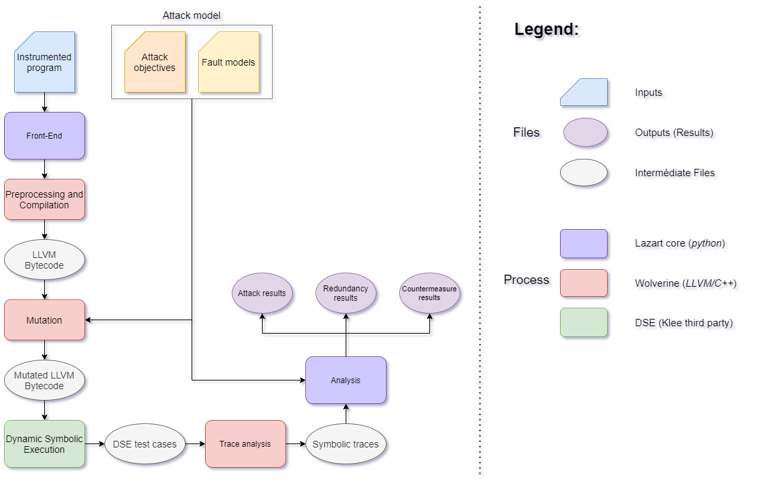
\includegraphics[width=\textwidth]{img/lazart-arch.png}
    \end{figure}
\end{frame}
    
\begin{frame}[fragile, noframenumbering]{Model protectability} 
    \begin{tiny}
        \begin{figure}
            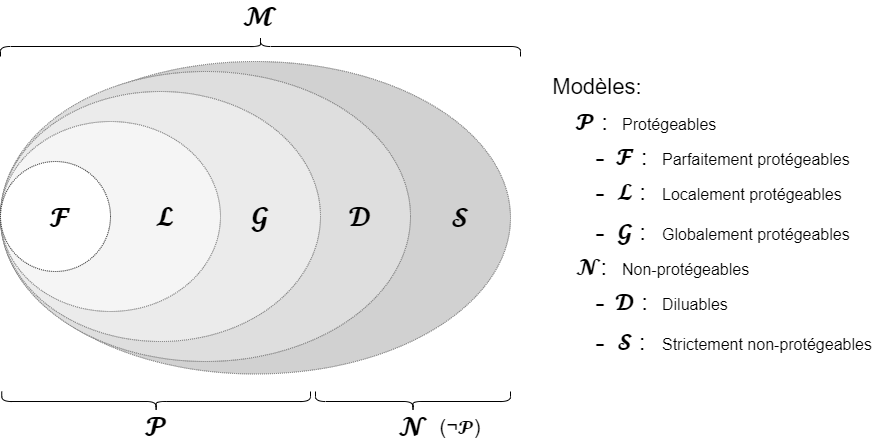
\includegraphics[scale=0.32]{img/protectable-models-set-extended.drawio.png}
        \end{figure}

        \begin{itemize}
            \item notion of \textit{adequation} of CMs
            \item notion of \textit{perfection} of CMs
            \item notion of protectability of models
        \end{itemize}
        \vfill
    \end{tiny}
\end{frame}

\begin{frame}[fragile, noframenumbering] \frametitle{Future work - Fully symbolic CCPO} 
    \begin{itemize}
        \item The methodology requires properties for detectors $\rightarrow$ a full symbolic version can be used
        \item[]
        \item Each detectors forks the execution:
        \lstset{style=customc}
        \begin{lstlisting}
if(sym_bool()) // Is the detector active ?
{
    // Local code with detector
}
else
{
    // Local unprotected code.
}
        \end{lstlisting}
        \item[]
        \item Issues:
        \begin{itemize}
            \item Paths explosion
            \item Some countermeasure structures depend on the presence of detectors (can require specific instrumentation for CMs)
        \end{itemize}
        \item[]
    \end{itemize}
\vfill
\end{frame}

\begin{frame}[fragile, noframenumbering]{Detector requirements} 
    \begin{itemize}
       \item[] Let $V_P$ be the state of the non-protected program and $V_C$ the state of the countermeasures.
       \item[] The detector has limitation for the read and write operation on the states $V_P$ et $V_C$.
    \end{itemize}
    
    \lstset{style=customc}
    \lstset{escapeinside={<@}{@>}, caption=Generic detector example}
    \begin{lstlisting}
...
stm1; // can: read(VP, VC) & write(VP, VC)

// Detector:
if(cond) { // read(VP, VC)
    stm2; // read(VP, VC) & write(VP, VC)
    killcard(); 
} 

stm3; // read(VP, VC) & write(VP, VC)
...
    \end{lstlisting}
\end{frame}

\begin{frame}[fragile, noframenumbering]{\texttt{memcmps3} program} 
    \begin{columns}
        \begin{column}{0.5\textwidth}
            \lstset{style=customc}
            \lstset{escapeinside={<@}{@>}, caption=Analysis's \texttt{main}}
            \begin{lstlisting}
// main.c
#include "lazart.h"
#include "memcmps.h"

#define SIZE 4

int main()
{  
    // Inputs
    uint8_t a1[SIZE];
    _LZ__SYM(a1, SIZE); // Symbolic array
    uint8_t a2[SIZE];
    _LZ__SYM(a2, SIZE); // Symbolic array
    
    bool equals = true;
    for(size_t i = 0; i < SIZE; ++i)
        if(a1[i] != a2[i])
            equals = false;
    _LZ__ORACLE(!equal); // Consider only different inputs
    
    BOOL res = memcmps(a1, a2, SIZE); // Call studied function

    _LZ__ORACLE(res == TRUE); // Attack objective
}
            \end{lstlisting}
        \end{column}
        \begin{column}{0.5\textwidth}
            \lstset{style=customc}
            \lstset{escapeinside={<@}{@>}, caption=\texttt{memcmps3} program}
            \begin{lstlisting}
// memcmps.h
typedef BOOL uint16_t;
#define TRUE    0x1234u
#define FALSE   0x5678u
#define MASK    0xABCDu

// memcmps.c
#include "memcmps.h"

BOOL memcmps(uint8_t* a, uint8_t* b, size_t len)
{
  BOOL result = FALSE;
  
  if (!memcmp(a, b, len)) {
    result ^= MASK;           // result = FALSE ^ MASK
    if (!memcmp(a, b, len)) {
      result ^= FALSE ^ TRUE; // result = MASK ^ TRUE
      if (!memcmp(a, b, len)) {
        result ^= MASK;       // result = TRUE
      }
    }
  }

  return result;
}
            \end{lstlisting}
        \end{column}
    \end{columns}
\end{frame}

\begin{frame}[fragile, noframenumbering]{\texttt{memcmps3} analysis file} 
    \lstset{style=custompython}
    \lstset{escapeinside={<@}{@>}, caption=\texttt{memcmps3} program}
    \begin{lstlisting}
#!/usr/bin/python3
from lazart.lazart import *

attack_model = functions_list(["memcmps"], [ti_model(), data_model({ "vars": { "result": "__sym__", "len":  "__sym__" } })])

a = Analysis(["memcmps.c", "main.c"], # Input files 
    attack_model, # Attack model
    flags=AnalysisFlag.AttacksAnalysis, # Analysis type
    compiler_args="-Wall",
    max_order=4,
    path="my_analysis")

execute(a)
    \end{lstlisting}
\end{frame}

\begin{frame}[fragile, noframenumbering]{Countermeasure optimization} 
    \begin{small}
        \begin{itemize}
            \item The program $P$ contains a set of \textit{detector} $\mathcal{D}$. 
            \item[]
            \item[] Stopping traces: $s_0 ... s_n d_i$, where $s_i$ are nominal or faulty transitions, and $d_i$ the triggered detector
            \item[] Non-stopping traces: $s_0 ... s_n d_i s^2_0 ... s^2_n d_j ...$ with $d_i$ detectors triggering
            \item[] $\rightarrow$ Stopping traces are prefix of non-stopping ones. One stopping trace can lead to several non-stopping traces
            \item [] 
            \item \textbf{Goal} $\Rightarrow$ find the minimal set of detectors in which at least one detector is kept for each trace
            \item [] 
            \item Only traces which validate the attack objective $\phi$ and in which at least one detector is triggered are considered. This trace set is denoted $\mathcal{T}_P$.
            \item[] The detector \textit{selection} is an optimization problem, searching a minimal set of detectors covering each traces of $\mathcal{T}_P$ with at least one trigger.
            \item[] Exploration space can be reduced:
            \begin{itemize}
                \item If $\forall t \in T', d_i \not\in  \{triggered(t)\}$, $d_i$ is inactive (should be removed)
            \item If $\exists t \in T', triggered(t) = \{d_i\}$, $d_i$ is necessary (should be kept)
            \end{itemize}
        \end{itemize}
    \end{small}
\end{frame}

\begin{frame}[noframenumbering]{Experimentation results - Playing with the attack objectives} 
    \only<1>{
        \vspace{0.6cm}
        The \textbf{attack objective} strongly impacts the removed \textbf{detectors}.
        
        \begin{itemize}
            \item []
            \item $\phi_{auth}$: being authenticated with a false PIN.
            \item $\phi_{ptc}$: do not decrement the try counter with a false PIN.
        \end{itemize}
        
        \begin{center}    
            \begin{table}[!t]
                \caption{Removed detectors depending on attack objective (VP + TD)}
                \centering
                \label{tbl:oracles}
                \begin{tabular}{|l|c|c|c|}
                    \hline
                    Property     & \multicolumn{1}{l|}{1 fault} & \multicolumn{1}{l|}{2 faults} & \multicolumn{1}{l|}{3 faults} \\ \hline
                    $\phi_{auth}$         & 83\%                         & 72\%                          & 18\%                          \\ \hline
                    $\phi_{ptc}$          & 72\%                         & 63\%                          & 9\%                           \\ \hline
                    $\phi_{auth\; \wedge \;ptc}$ & 83\%                         & 72\%                          & 18\%                          \\ \hline
                    $\phi_{auth\; \vee \;ptc}$  & 72\%                         & 63\%                          & 9\%                           \\ \hline
                    $\phi_{true}$         & 18\%                         & 9\%                           & 9\%                           \\ \hline
                \end{tabular}
            \end{table}
        \end{center}
        \vfill
    }
\end{frame}

\begin{frame}[fragile, noframenumbering]{Test Duplication} 
    The \textit{Test Duplication} generate two detectors for each conditional branch.

    \vspace{0.5cm}

    \begin{figure}
        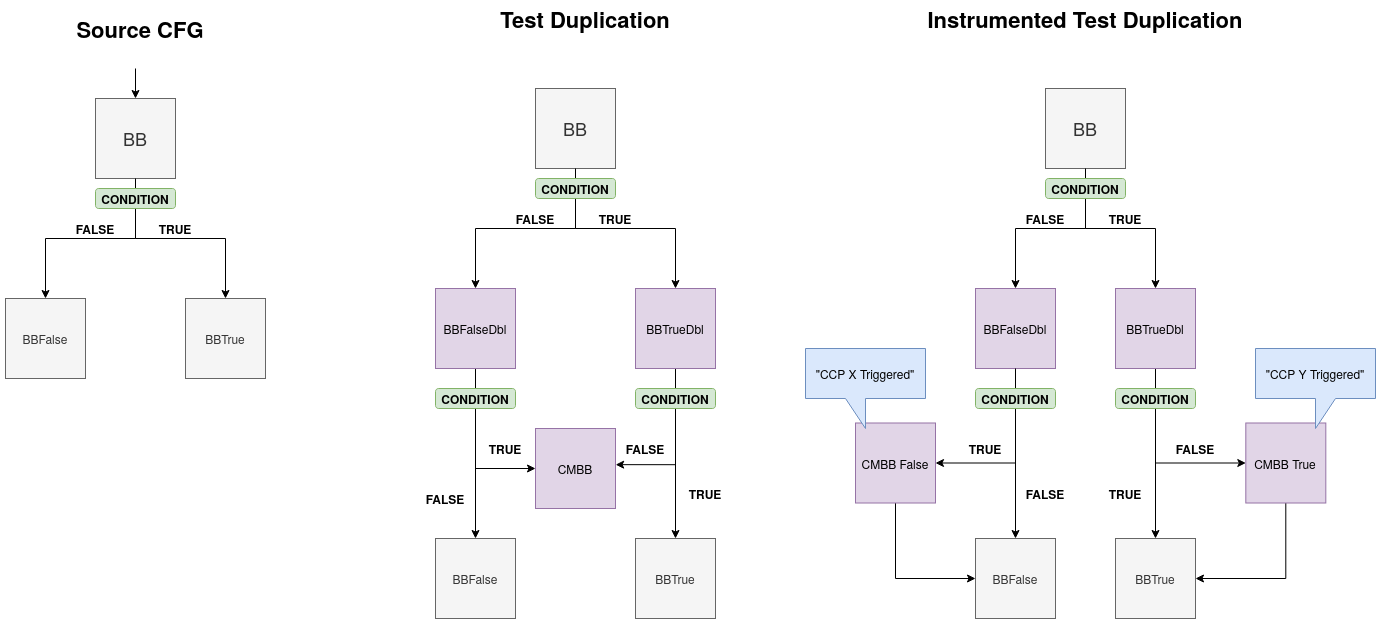
\includegraphics[scale=0.2]{img/test-duplication-scheme-complete-old.png}
    \end{figure}
\end{frame}

\begin{frame}[fragile, noframenumbering]{SecSwift Control-Flow} 
    \begin{figure}
        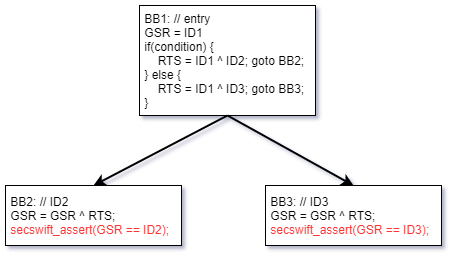
\includegraphics[scale=0.3]{img/secswift-CF.png}
    \end{figure}
    
    \begin{itemize}
        \item []
        \item[] SecSwift ControlFlow is one of the 3 parts of SecSwift\cite{Ferriere/LLVM19}
        \item []
        \item Designed for Control-Flow Integrity (CFI)
        \item[]
        \item Uses static signature for each basic block and propagate errors
        \item[]
        \item Each \lstinline{secswift_assert} is a \emph{detector}
    \end{itemize}
    \vfill
\end{frame}

\begin{frame}[fragile, noframenumbering]{LBH's countermeasure \cite{Lalande/ESORICS14}} 
    \vspace{0.3cm}
    
    \lstset{style=customc}
    \lstset{escapeinside={<@}{@>}}
    \begin{lstlisting}
#define <@{\color{red!95} INCR}@>(cnt,val)  cnt = cnt + 1;
#define <@{\color{red!95} CHECK\_INCR}@>(cnt,val, cm_id) if(cnt != val) countermeasure(cm_id); \
    cnt = cnt + 1;
[...]
        
        
BOOL verifyPIN(<@{\color{red!95}unsigned short* CNT\_0\_VP\_1}@>) 
{
    <@{\color{red!95} CHECK\_INCR(*CNT\_0\_VP\_1, CNT\_INIT\_VP + 0, 0LL)}@>
    g_authenticated = 0;
    <@{\color{red!95} CHECK\_INCR(*CNT\_0\_VP\_1, CNT\_INIT\_VP + 1, 1LL)}@>
    <@{\color{red!95} DECL\_INIT(CNT\_0\_byteArrayCompare\_CALLNB\_1, CNT\_INIT\_BAC)}@>
    <@{\color{red!95} CHECK\_INCR(*CNT\_0\_VP\_1, CNT\_INIT\_VP + 2, 2LL)}@>
    BOOL res = byteArrayCompare(g_userPin, g_cardPin, PIN_SIZE<@{\color{red!95}, \&CNT\_0\_byteArrayCompare\_CALLNB\_1}@>);
[...]
    \end{lstlisting}

    \begin{itemize}
        \item Insert \textit{step-counters} for each C construct
        \item[]
        \item \textit{Checking macros} (such as \lstinline{CHECK_INCR}) are \emph{detectors}
        \item[]
        \item Analysis allows to know where the counter verification can be removed
    \end{itemize}
    \vfill
\end{frame}